\newpage
\hypertarget{sec:conBran}{}
\section{Conditional branching}
\genHeader

When working with SDMs, you'll often find yourself needing to decide which statement(s) to execute based on the return value of an arbitrary (black box)
operation, as we saw in \texttt{check}. In our example so far, we have implemented these constructs via SDM \emph{pattern matching}. 

With eMoflon however, there is an alternate way to construct these black boxes. In fact, this feature is yet another way of integrating handwritten java code
with your SDM. We can invoke methods directly from an \emph{if} statement. The only ``rule'' of this feature is that the method must return an
\texttt{EBoolean} to indicate \texttt{Success} or \texttt{Failure}, corresponding to \texttt{true} or \texttt{false}, respectively. Any other types imply
\texttt{Failure} if the return value of the method is \texttt{null}. It follows that void methods cannot be used for branching -- an exception will be thrown
during code generation (if you ignored the validation error).

Unfortunately, you can't simply invoke a method from a standard activity node. Instead, you must use a new type of activity node, a \emph{statement
node}.\define{Statement Node}Statement nodes can be used to invoke methods and provide a means of invoking libraries and
arbitrary Java code from SDMs. Please note that we do not differentiate at this point between methods that are implemented by hand or via an SDM. Thus,
statement nodes can of course be used to invoke other SDMs via a \emph{MethodCallExpression}. Most importantly, statement nodes enable \emph{recursion}, as the
current SDM can be invoked on \texttt{this} with appropriate new arguments. In essence, this type of node is only used to guarantee a specific action
between \emph{activity nodes}, and does not extend the current set of matched variables. They can however, be used as a conditional by branching on
whatever value the method returns.

Let's reconsider \texttt{grow}, the method we just completed that adds a new partition to our box. Reviewing either Fig.~\ref{fig:growComplete} (Visual) or
Fig.~\ref{fig:patternComplete} (Textual), the current pattern assumes there are already at least two partitions in \texttt{box} (the
\texttt{firstPartitionInBox} and \texttt{LastPartitionInBox}). What would happen if \texttt{box} had only one, or even no partitions at all? The pattern would
\emph{never} find a match!

To fix this problem, let's modify \texttt{grow} so that if the original match fails, we initialize two new partitions (the first and last), but \emph{only} if
it failed due to the box being completely empty. In other words, if \texttt{box} has e.g., only one partition (an invalid state that cannot be reached by
growing from zero partitions), it is considered invalid and no longer be grown.

\jumpDual{conBran vis}{conBran tex}

\clearpage
\hypertarget{conBran vis}{}
\subsection{Branching with statement nodes}
\visHeader

\begin{itemize}
  
\item[$\blacktriangleright$] Edit the \texttt{Box} class in your metamodel by invoking the \texttt{Operations} dialogue and create a new method called
\texttt{initalizeBox}. Recalling the sole condition of conditional branching, set its return type to \texttt{EBoolean}. Save the method, then re-open the
\texttt{grow} SDM.

\vspace{0.5cm}

\item[$\blacktriangleright$] Add a new \texttt{StatementNode} from \texttt{addNewPartitionBox} and name it \texttt{initialize}. The edge guard should
automatically set itself to \texttt{failure}.

\vspace{0.5cm}

\item[$\blacktriangleright$] In the \texttt{Statement} tab, invoke a \texttt{MethodCallExpression} to your new method.

\vspace{0.5cm}

\item[$\blacktriangleright$] Finally, attach two \texttt{StopNode}s -- \texttt{true} and \texttt{false} -- along with their appropriate edge guards. These mean
that the if method call succeeds, the box could be initialized, so it will return a literal \texttt{true}. If it failed however, \texttt{box} was already in an
invalid state (by, i.e., having only one card) and returns \texttt{false}. Overall, the new additions to \texttt{box.grow()} should resemble
Fig.~\ref{fig:newGrowControl}.

\vspace{0.5cm}

\begin{figure}[htp]
\begin{center}
  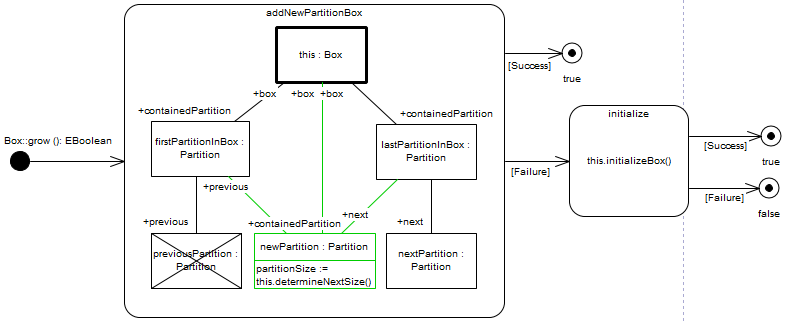
\includegraphics[width=\textwidth]{ea_growAdditions}
  \caption{Extending \texttt{grow} with a \emph{MethodCallExpression}}
  \label{fig:newGrowControl}
\end{center}
\end{figure}

\clearpage

\item[$\blacktriangleright$] Switch back to your open \texttt{Box.grow} SDM in EA. You'll notice that if you double-click on \texttt{initialize}, the
\texttt{Extract Story Pattern} option is invalid. This makes sense -- you don't define a pattern in a statement node. Instead, return to the main diagram and
create a new SDM for \texttt{initializeBox}.

\item[$\blacktriangleright$] In its diagram, create an \texttt{activity node} named \texttt{buildPartitions}. Within it, have a bound \texttt{Box} linked to a
\texttt{onePartition} NAC, and two other `green' (create) object variables, \texttt{firstPartition} and \texttt{lastPartition}. Be sure to also connect two
true/false \texttt{StopNode}s. The pattern should now resemble Fig.~\ref{fig:buildPartitions}. The NAC here can only fulfilled if the box has no partitions,
i.e., is in a pristine state and able to be initialized. In other words, If \texttt{grow} is used for an empty box, it initializes the box for the first time
and grows it after that, ensuring that the box is always in a valid state.

\vspace{0.5cm}
 
\begin{figure}[htp]
\begin{center}
  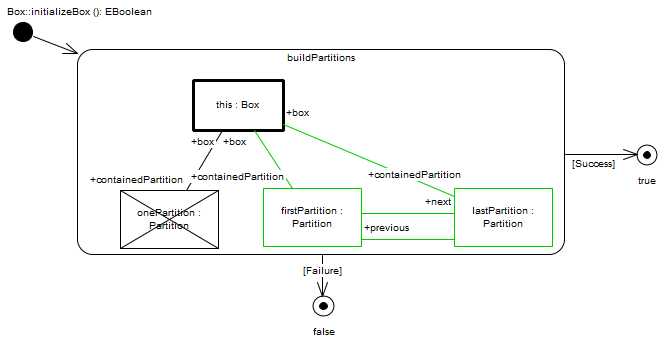
\includegraphics[width=\textwidth]{eclipse_buildPartitions}
  \caption{Compelted NAC to check for \emph{one} partition}
  \label{fig:buildPartitions}
\end{center}
\end{figure}
 
\item[$\blacktriangleright$] You're finished! Save, validate, and build your metamodel, then check out how this is done in the textual syntax in
Fig.~\ref{fig:updateGrow} and Fig.~\ref{fig:pattBuildParts}.

\jumpSingle{initialize notes}

\end{itemize}


\newpage
\hypertarget{conBran tex}{}
\subsection{Branching with statement nodes}
\texHeader

\begin{itemize}

\item[$\blacktriangleright$] Before doing anything else, let's declare the method that will insert two new partitions into \texttt{box} when the original
pattern match fails. Open \texttt{Box.eclass} and add the following signature anywhere in the file: 
\syntax{initializeBox() : EBoolean}

\vspace{0.5cm}

\item[$\blacktriangleright$] Now modify \texttt{Box.grow()} by adding a nested \emph{if/Else} construct, with \texttt{[addNewPartitionBox]} as the
first conditional, and execute a \emph{statement node} if it fails. \texttt{grow} should now resemble Fig.~\ref{fig:updateGrow}.

\vspace{0.5cm}

\begin{figure}[htp]
\begin{center}
  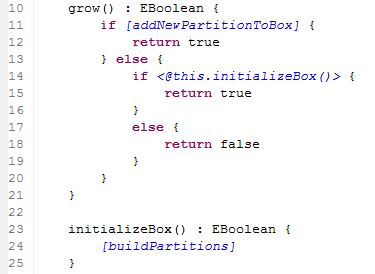
\includegraphics[width=0.5\textwidth]{eclipse_updateGrow}
  \caption{Extending \texttt{Box} with a \emph{statement node}}
  \label{fig:updateGrow}
\end{center}
\end{figure}

\vspace{0.5cm}

\item[$\blacktriangleright$] Next, we want to specify our newest method. Create a new pattern called \texttt{buildPartitions} in its scope. Complete
the pattern as illustrated in Fig.~\ref{fig:pattBuildParts}.

\item[$\blacktriangleright$] As you can see, we have created a NAC that can only be fulfilled if the box has no lonely partition. In turn, this means that if a
box is completely empty, it will be intialized for the first time with two partitions, and guaranteed to remain in a valid state if growing continues.

\clearpage

\vspace*{2cm}

\begin{figure}[htp]
\begin{center}
  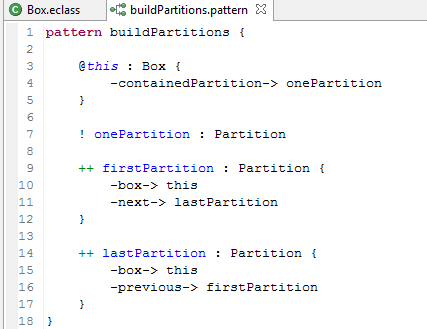
\includegraphics[width=0.7\textwidth]{eclipse_buildPartitionsPattern}
  \caption{NAC initalizing an empty box}
  \label{fig:pattBuildParts}
\end{center}
\end{figure}

\item[$\blacktriangleright$] That's it! Save and build your metamodel to make sure no errors exist. To see how this is depicted in the visual syntax, check out
Fig.~\ref{fig:newGrowControl} and Fig.~\ref{fig:buildPartitions}.

\end{itemize}


\newpage
\hypertarget{initialize notes}{}
\subsection{A short note on the \texttt{initializeBox} method}
\genHeader

Pretend you've just updated the control flow in your \texttt{grow} SDM, and haven't specified \texttt{initializeBox} yet. After saving and building, you will be
able to see the changes in \texttt{BoxImpl.java}, the source file containing the generated code. In fact, open this file now and navigate to \texttt{grow},
which starts at (approximately) line 207 (Fig.~\ref{eclipse:initBoxImpl}). This is the generated \emph{statement node} code and, as you can see, all it does is
invoke your method and branch based on its result. 

\begin{figure}[htp]
\begin{center}
  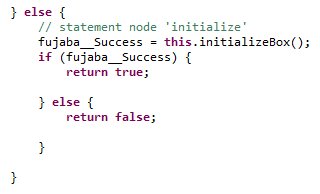
\includegraphics[width=0.5\textwidth]{eclipse_boxImplStatementNode}
  \caption{Code generated for branching with a statement node}
  \label{eclipse:initBoxImpl}
\end{center}
\end{figure}

Hold \texttt{ctrl} while clicking on \texttt{initializeBox()} to automatically jump to its declaration. If you didn't complete the SDM, it
would look like Fig.~\ref{eclipse:initBoxDecl}.

\begin{figure}[htp]
\begin{center}
  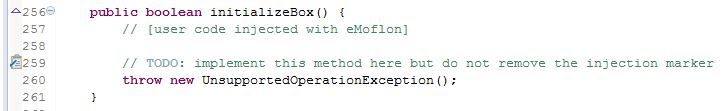
\includegraphics[width=\textwidth]{eclipse_initializeBoxDeclaration}
  \caption{The \texttt{initializeBox} declaration}
  \label{eclipse:initBoxDecl}
\end{center}
\end{figure}

You have the choice of either implementing the method by hand here in Java as an injection, or you can return to the metamodel and implement it there as an SDM.
The statement node will work just fine in both cases.

Using Java and injections makes sense if the method is non-structural, but seeing as we must check to see if there is a single partition, then create the
first two partitions of the box if it succeeds, \texttt{initializeBox} is actually quite structural and can be described beautifully as a pattern. This is why
we opted to specify it as an SDM.


